\documentclass[tikz,border=5mm]{standalone}
\usepackage{amsmath}
% Librerías de TikZ necesarias para posicionamiento, cálculo de coordenadas y la caja exterior
\usetikzlibrary{positioning, calc, fit, arrows.meta, backgrounds}

\definecolor{MiAzul}{cmyk}{1.00,0.2,0,0.87}

\begin{document}

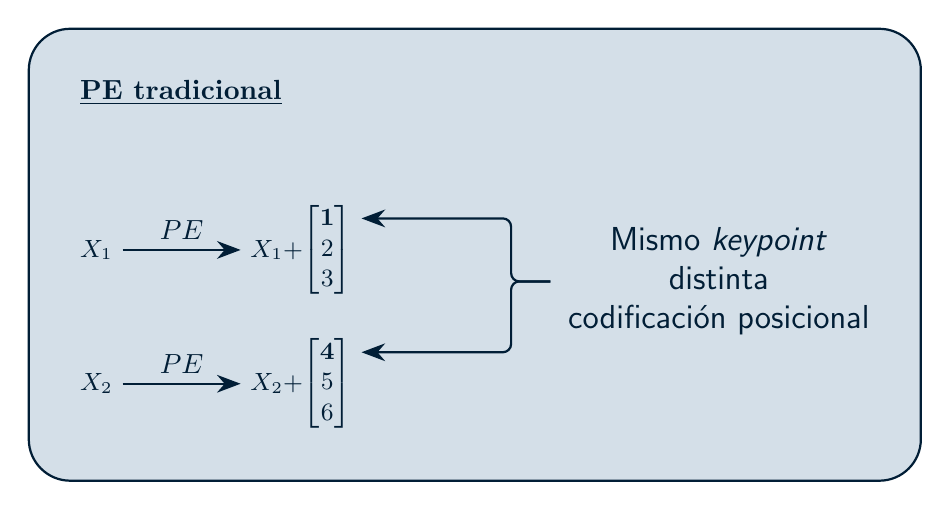
\begin{tikzpicture}[
%     background rectangle/.style={fill=MiAzul!30},
%     show background rectangle,
%     inner frame sep=0pt,
    >={Stealth[length=3mm]}, % Estilo de flecha más definido
    texto/.style={font=\sffamily\large, align=center},
    mathnode/.style={font=\small},
    color_tinta/.style={color=MiAzul} % Color inspirado en tu apunte
]

    % 1. Título y Definición principal (Parte superior)
    \node[color_tinta] (titulo) {\underline{\textbf{PE tradicional}}};
    %\node[mathnode, below right=-0.75cm and 3cm of titulo, color_tinta] (def) {$X = [X_1, X_2], \quad X_i = \begin{bmatrix} p_1^i \\ \vdots \\ p_3^i \end{bmatrix}$};

    % 2. Transformación 1 (Medio)
    \node[mathnode, below=2cm of titulo.west, anchor=west, color_tinta] (x1) {$X_1$};
    \node[mathnode, right=1.5cm of x1, color_tinta] (x1_add) {$X_1 +$};
    \draw[->, color_tinta, thick] (x1) -- node[above] {$PE$} (x1_add);
    \node[mathnode, right=-0.25cm of x1_add, color_tinta] (vec1) {$\begin{bmatrix} \mathbf{1} \\ 2 \\ 3 \end{bmatrix}$};

    % 3. Transformación 2 (Abajo)
    \node[mathnode, below=1.2cm of x1, color_tinta] (x2) {$X_2$};
    \node[mathnode, right=1.5cm of x2, color_tinta] (x2_add) {$X_2 +$};
    \draw[->, color_tinta, thick] (x2) -- node[above] {$PE$} (x2_add);
    \node[mathnode, right=-0.25cm of x2_add, color_tinta] (vec2) {$\begin{bmatrix} \mathbf{4} \\ 5 \\ 6 \end{bmatrix}$};

    % 4. Nota explicativa lateral
    \node[texto, right=2.5cm of vec1, yshift=-0.4cm, color_tinta] (nota) {Mismo \textit{keypoint} \\ distinta\\ codificación posicional};

    \coordinate[left=0.6cm of nota] (joint);
    % 5. Flechas conectando la nota con las matrices de los vectores
    % El uso de |- crea líneas con un quiebre de 90 grados (primero horizontal, luego vertical)
    \draw[->, color_tinta, thick, rounded corners=3pt] ($(joint.east) + (0.5,0)$) -- ++(-0.5,0) |- ($(vec1.east) + (0, 0.4)$);
    \draw[->, color_tinta, thick, rounded corners=3pt] ($(joint.east) + (0.5,0)$) -- ++(-0.5,0) |- ($(vec2.east) + (0, 0.4)$);

    % 6. Caja contenedora exterior
    % La librería 'fit' envuelve automáticamente todos los nodos listados
    \begin{scope}[on background layer]
        \node[draw, fill=MiAzul!10, draw=MiAzul, thick, rounded corners=15pt, inner sep=15pt, fit=(titulo) (x2) (vec2) (nota)] (caja) {}; %(def)
     \end{scope}

\end{tikzpicture}

\end{document}
